\documentclass[10pt]{article}
\usepackage[T1]{fontenc}
\usepackage[utf8]{inputenc}
\usepackage[polish]{babel}
\usepackage{amsthm}
\usepackage{amsfonts}
\usepackage{titlesec}
\usepackage{graphicx}
\title{%
  Sprawozdanie \\
  \large P1.8 z analizy numerycznej\\
    obliczanie wartości logarytmu naturalnego}
\author{Mateusz Markiewicz}
\begin{document}
\maketitle
\tableofcontents

\newtheorem{definition}{Definicja}[section]

\titleformat{\paragraph}
{\normalfont\normalsize\bfseries}{\theparagraph}{1em}{}
\titlespacing*{\paragraph}
{0pt}{3.25ex plus 1ex minus .2ex}{1.5ex plus .2ex}

%~~~~~~~~~~~~~~~~~~~~~~~~~~~~~~~~~~~~~~~~
\newpage
\section{Wstęp}
\subsection{Cel zadania}
Celem zadania jest doświadczalne zbadanie jak dobre przybliżenie wartości $\ln x$ dla $ x \in [\frac{1}{2},1]$ otrzymamy obliczając ją za pomocą wyrażenia: \\
\\

\begin{math}
-\frac{1}{2} \ln2 + \sum_{k=0}^{3} a_{2k+1} \left(\frac{x - \frac{\sqrt{2}}{2}}{x + \frac{\sqrt{2}}{2}} \right)^{2k+1}
\end{math} , gdzie: \\
a1 := 1.999999993788, \hspace{1.5cm} a3 := 0.399659100019, \\
a5 := 0.666669470507, \hspace{1.5cm} a7 := 0.300974506336. \\
\\
Na podstawie tego należy zaproponować metodę o podobnej dokładności umożliwiającą obliczanie logarytmu naturalnego dla $x>0$.
\subsection{Streszczenie sprawozdania}
Sprawozdanie będzie składać się z trzech głównych części. Pierwsza z nich będzie skupiać się na teoretycznym wprowadzeniu do problemu obliczania wartości logarytmu naturalnego danej liczby. W drugiej części zostanie zbadana dokładność metody zaprezentowanej jako cel zadania, co zostanie wykorzystane w części trzeciej skupiającej się na rozbudowie metody w sposób umożliwiający obliczanie logarytmu naturalnego z dowolnego $x >0$.Zaproponowana metoda zostanie porównana z funkcją biblioteczną.\\


\section{Opis teoretyczny problemu}

\subsection{Logarytm naturalny}
Logarytm naturalny liczby x $(\ln x)$, czyli logarytm o podstawie e liczby x, gdzie e jest liczbą Eulera, to funkcja matematyczna wyznaczająca liczbę równą potędze do której należy podnieść podstawę logarytmu (czyli w naszym przypadku liczbę Eulera) by wynik wynosił x. \\
\theoremstyle{definition}
\begin{definition}{Logarytm naturalny}
\begin{math}
\ln(x) = c \Longleftrightarrow e^c = x,
\end{math}
gdzie $e \approx 2,718281828459$
\end{definition}

\subsection{Problem obliczania logarytmu naturalnego}
Ciężko wskazać jednoznacznie najlepszą metodę wyznaczania logarytmu naturalnego danej liczby. Dobór odpowiedniej metody zależy od wymaganej dokładności obliczeń, szybkości wyznaczenia oraz wielkości liczby której logarytm chcemy obliczyć. Poniżej przedstawię kilka stosowanych metod obliczania $\ln x$.\\

\paragraph{Metoda Newtona}

Metoda Newtona służy do znajdowania miejsca zerowego funkcji nieliniowej f. Jeśli ustalimy funkcję f taką, że jej miejscem zerowym będzie wartość $\ln x$ metoda Newtona pozwoli nam wyznaczyć przybliżenie tej wartości. Metoda ta wykorzystuje styczne do przybliżania miejsca zerowego funkcji. Mając już jakieś przybliżenie miejsca zerowego metoda Newtona pozwala nam znacznie zwiększyć dokładność przybliżenia tej wartości w stosunkowo krótkim czasie, przez co często stosuje się ją w połączeniu z innymi metodami.\\
$f(x)$ - funkcja, której miejscem zerowym jest $\ln x$, $f \in C^{2}$ \\
$x_{0}$ - przybliżenie początkowe \\
$x_{n+1} = x_{n} - \frac{f(x_{n})}{f'(x_{n})}$\\
Chcąc obliczyć $ln(a)$ jako $f(x)$ można wziąć funkcję $f(x) = e^{x} - a$, stąd $f'(x) = e^{x}$. Dzięki temu uzyskujemy następujący wzór na następne przybliżenie $x_{n}$:\\
$x_{n+1} = x_{n} - 1 + \frac{a}{e^{x_{n}}}$


\paragraph{Rozwinięcie $\ln x$ w szereg Taylora}

Prostą, ale jednocześnie mało dokładną metodą obliczania $\ln x$ dla $x \in (0,2)$ jest obliczanie go z rozwinięcia logarytmu w szereg Taylora.\\

\begin{math}
\ln x = \sum_{i=1}^\infty
(-1)^{i+1} \frac{(x-1)^{i}}{i}
\end{math} \\

\paragraph{Funkcje hiperboliczne odwrotne}

Inną używaną metodą jest obliczanie logarytmu używając funkcji hiperbolicznych odwrotnych. Pozwala to na obliczenie logarytmu naturalnego z dowolnego $ x > 0 $.\\

\begin{math}
\ln x = 2 \sum_{i=0}^\infty
\frac{1}{2i + 1} \left(\frac{x-1}{x+1} \right)^{2i+1}
\end{math} \\

Powyższa metoda zbiega szybciej, niż szereg Taylora i jest dokładna, szczególnie dla x bliskiego 1. Fakt ten jest wykorzystywany do uzyskiwania kolejnych, bardziej skomplikowanych ale również bardziej dokładnych metod obliczania logarytmu naturalnego.\\
Chcąc obliczyć $\ln x$ dla $x >> 1$ możemy wyznaczyć mało dokładne przybliżenie $y \approx \ln x$. Dzięki temu możemy wyznaczyć liczbę $a = \frac{x}{e^{y}}$, której wartość jest bliska 1. Dzięki temu metoda funkcji hiperbolicznych odwrotnych będzie szybka i dokładna. Następnie korzystając z własności logarytmów obliczamy: \\
$\ln x = y + \ln a$\\

%~~~~~~~~~~~~~~~~~~~~~~~~~~~~~~~~~~~~~~~~

\section{Doświadczalne wyznaczenie dokładności badanej metody obliczania $\ln x$}
\subsection{Wstęp i plan obliczeń}
Niech 
\begin{math}
f(x) = -\frac{1}{2} \ln2 + \sum_{k=0}^{3} a_{2k+1} \left(\frac{x - \frac{\sqrt{2}}{2}}{x + \frac{\sqrt{2}}{2}} \right)^{2k+1}
\end{math} , gdzie: \\
\\
a1 := 1.999999993788, \hspace{1.5cm} a3 := 0.399659100019, \\
a5 := 0.666669470507, \hspace{1.5cm} a7 := 0.300974506336. \\
\\
By sprawdzić jak dokładnym przybliżeniem $\ln x$ jest $f(x)$ porównam wartość $f(x)$ z wartością funkcji bibliotecznej $\ln x$ w N równo oddalonych punktach z przedziału $[\frac{1}{2},1]$. \\
Do obliczeń użyję programu w języku Julia w wersji 1.0.1. Liczby zmiennoprzecinkowe reprezentowane będą w podwójnej precyzji. 

\subsection{Prezentacja wyników}
Dokładność wyników prezentowana jest jako ilość cyfr znaczących wyniku. Jako wartość dokładną uznaję wartość obliczoną za pomocą funkcji bibliotecznej. Ilość cyfr znaczących obliczam za pomocą wzoru: \\
\\
\begin{math}
-log_{10}(|\frac{x-x0}{x0}|)
\end{math}, gdzie x0 - wartość dokładna, x - wartość obliczona\\

Poniższy wykres przedstawia ilość cyfr znaczących uzyskanych obliczając $\ln(x)$ za pomocą badanej metody w 50 równo odległych punktach z przedziału $[\frac{1}{2},1]$.\\

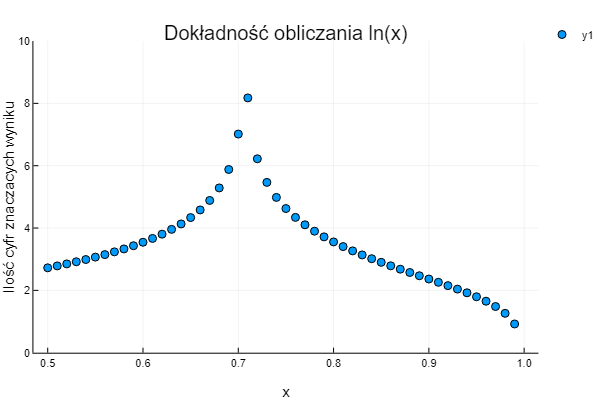
\includegraphics[scale=0.60]{wykres1.png}


\subsection{Wnioski}
Badany sposób pozwala nam uzyskać wynik z dokładnością od 2 do 8 miejsc znaczących względem wartości dokładnej. Największą dokładność uzyskujemy dla wartości $x \approx 0.7$. Zarówno dla $x > 0.7$ jak i $x < 0.7$ dokładność maleje, by dla $x = 0.5$ oraz $x = 1$ wynieść 2 cyfry znaczące. Można również zauważyć, że dokładność obliczeń dla $x \approx 1$ jest według wykresu mniejsza, niż dla $x \approx 0.5$. Wynika to jednak nie z dokładności badanej metody lecz ze sposobu obliczania ilości cyfr znaczących wyniku. Dla $x \approx 1$ $\ln(x) \approx 0$, stąd wartość $-log_{10}(|\frac{x-x0}{x0}|)$ może być bardzo mała.\\ 

%~~~~~~~~~~~~~~~~~~~~~~~~~~~~~~~~~~~~~~~~

\section{Propozycja metody obliczania logarytmu naturalnego}
\subsection{Wstęp i przedstawienie metody}
Zaprezentowana wyżej metoda pozwala na obliczenie logarytmu naturalnego, lecz jedynie z $x \in [\frac{1}{2},1]$. W przypadku $x>0$ można jednak zastosować następującą metodę. \\
Dowolny $x \in (0,\infty)$ możemy przedstawić w postaci $x = y * 2^{i}$, gdzie $i \in \mathbb{Z}, y \in [\frac{1}{2},1)$. Korzystając z własności logarytmu:\\
\\
$\ln(x) = \ln(y*2^{i}) = \ln(y) + \ln(2^{i}) = \ln(y) + i\ln(2)$\\
Wartość $\ln(y)$ możemy obliczyć za pomocą wzoru: \\
\\
\begin{math}
\ln(y) = -\frac{1}{2} \ln2 + \sum_{k=0}^{3} a_{2k+1} \left(\frac{y - \frac{\sqrt{2}}{2}}{y + \frac{\sqrt{2}}{2}} \right)^{2k+1}
\end{math} , gdzie: \\
\\
a1 := 1.999999993788, \hspace{1.5cm} a3 := 0.399659100019, \\
a5 := 0.666669470507, \hspace{1.5cm} a7 := 0.300974506336. \\
\\
którego dokładność obliczeń dla wartości z przedziału $[\frac{1}{2},1)$ już znamy. Ostateczny wzór prezentuje się więc następująco: \\
\\
\begin{math}
\ln(x) = \ln(y*2^{i}) = (i -\frac{1}{2}) \ln2 + \sum_{k=0}^{3} a_{2k+1} \left(\frac{y - \frac{\sqrt{2}}{2}}{y + \frac{\sqrt{2}}{2}} \right)^{2k+1}
\end{math} , gdzie: \\
\\
a1 := 1.999999993788, \hspace{1.5cm} a3 := 0.399659100019, \\
a5 := 0.666669470507, \hspace{1.5cm} a7 := 0.300974506336. \\
\\


\subsection{Porównanie dokładności badanej metody z dokładnością funkcji bibliotecznej}
Badanie dokładności zmodyfikowanej metody obliczania $\ln(x)$ następuje w sposób analogiczny do tego z punktu 3. Sposób ten zostanie zastosowany na różnych przedziałach.

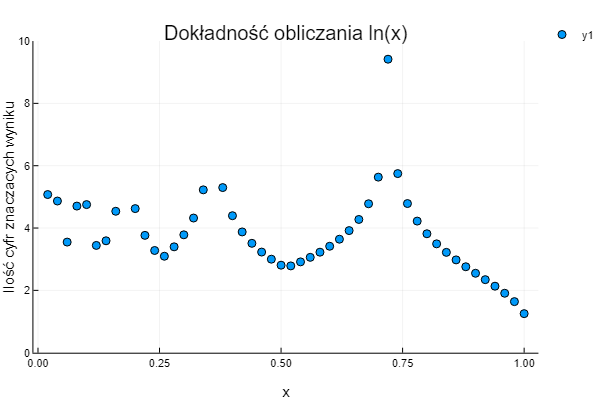
\includegraphics[scale=0.60]{wykres2.png}
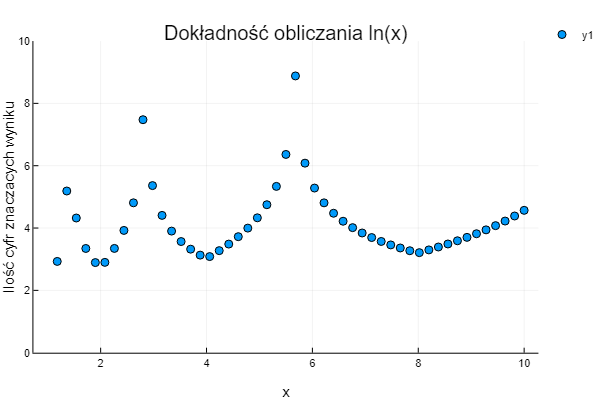
\includegraphics[scale=0.60]{wykres3.png}
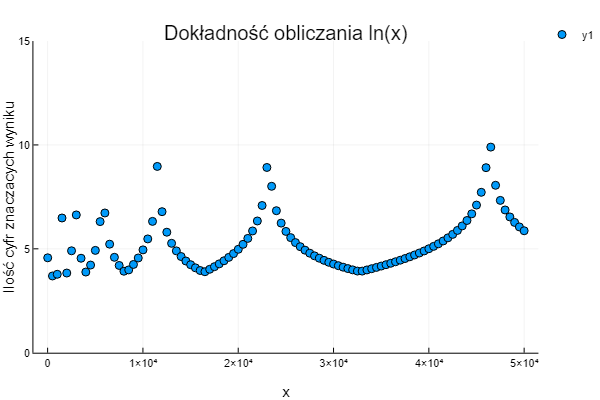
\includegraphics[scale=0.60]{wykres4.png}


\subsection{Wnioski}
Wartość $\ln(x)$ dla $x>0$ oblicza się ze średnią dokładnością 5 cyfr znaczących. To, ile cyfr znaczących otrzymamy zależy od wartości y w postaci $x = y * 2^{i}$, gdzie $y \in [\frac{1}{2},1), i \in \mathbb{Z}$. Jeśli $y \approx 0.7$ dokładność jest najwyższa, dla innych wartości y dokładność maleje. Na podstawie wykresów obserwujemy również, że wahania dokładności metody są cykliczne i wynika to bezpośrednio z zapisu w postaci $x = y * 2^{i}$.\\
W badanej metodzie obliczamy cztero­elementową sumę, dodając do niej pewną wielokrotność $\ln(2)$. Dzięki temu metoda ta pozwala szybko uzyskać wynik, lecz otrzymane wyniki nie mają dużej dokładności. Z tego powodu owa metoda sprawdzi się w przypadkach, gdy nie potrzebujemy wysokiej precyzji, a liczy się dla nas czas obliczeń.

%~~~~~~~~~~~~~~~~~~~~~~~~~~~~~~~~~~~~~~~~

\section{Podsumowanie}
Problem obliczania wartości logarytmu naturalnego z danej liczby jest skomplikowany, a sposobów jego rozwiązania jest wiele. Każdy z tych sposobów ma swoje wady i zalety. Badana metoda obliczania $\ln(x)$ za pomocą czteroelementowej sumy pozwala na szybkie uzyskanie wyniku ze średnią dokładnością 5 cyfr znaczących. Wiedząc to możemy wybrać tą metodę w sytuacjach, gdy taka dokładność wyniku jest dla nas satysfakcjonująca oraz w przypadkach gdy zależy nam na szybkości obliczeń. Należy również pamiętać, że dokładność 5 cyfr znaczących jest dokładnością średnią. Istnieją liczby których logarytm obliczymy z większą lub mniejszą dokładnością. 

\section{Literatura}

1) M. Dryja, J. i M. Jankowscy, Przegląd metod i algorytmów numerycznych, cz. 1 i 2, WNT, 1988.\\
2) D. Kincaid, W. Cheney, Analiza numeryczna, WNT, 2005.\\


\end{document}
